\chapter{Looking for Supercoiling Epistasis in \emph{Aevol}}
\label{chap:aevol}

In this chapter, I present the first main line of work of that I undertook during my Ph.D.
In order to understand the role of epistasis in the prediction of evolution, I focused on the study of the specific case of mutations affecting the DNA supercoiling level in bacteria, which were shown to be repeatable at the phenotypic level,  and partially repeatable at the molecular level, in an experimental evolution setting.
In order to replicate these results in the easier to study \emph{in silico} artificial evolution setting offered by the \emph{Aevol} software platform, I implemented a model of supercoiling in \emph{Aevol}, and tried to detect epistatic interactions in the evolutionary trajectories of populations evolved in the model.

\section{Introduction}
\label{sec:aevol:intro}

In the \emph{Long-Term Evolution Experiment} (LTEE), started by Richard Lenski in 1988~\citep{lenski1991}, 12 populations of \emph{E. coli} cells, originating from the same ancestral strain, were placed to evolve in a new environment, an Erlenmeyer flask containing a glucose-limited medium.
Every day since the beginning of the experiment, which is still running and has reached over 75,000 generations of bacteria, a sample from each population has been propagated into fresh medium, and samples have been cryogenically conserved every 500 generations, resulting in the longest-running evolution experiment in the lab.
The LTEE demonstrated that fitness can keep on increasing for much longer than originally expected in a constant environment~\citep{good2017}.
As sequencing capacity and synthetic biology subsequently developed in the late 1990s and early 2000s, identifying the precise DNA mutations underpinning these increases in fitness became possible.
When sequencing the conserved \emph{E. coli} lineages in the LTEE, beneficial mutations -- mutations that confer their bearer a higher growth rate than the ancestral strain in the conditions of the experiment -- were in particular found in the \emph{topA} gene  and the \emph{fis} gene, in one of the twelve lineages~\citep{crozat2005}.

The genes affected by these mutations are involved in the regulation of DNA supercoiling: Topoisomerase I (encoded by \emph{topA}) directly modifies the supercoiling level by introducing supercoils, and FIS (encoded by \emph{fis}) is a nucleoid-associated protein which helps regulate supercoiling by binding to DNA.
This makes these mutation extremely interesting in two regards.
First, there is no direct phenotypic link between the supercoiling level of the chromosome and the growth rate of the bacteria, and yet these mutations, when inserted into the genetic background of the ancestral strain, still confer a fitness advantage.
Second, mutations affecting supercoiling-regulating genes, especially in \emph{gyrA} and \emph{fis}, were subsequently found in 11 of the 12 replicates of the experiment after 20,000 generations of evolution, a rate that is much higher than for randomly chosen genes~\citep{crozat2010}.
A possible interpretation of this repeated mutational targeting of supercoiling-regulating genes is that, by globally altering the transcriptional landscape of the bacteria (as the level of supercoiling directly affects gene transcription), these mutations enable the exploration of new evolutionary pathways that would have been deleterious in the ancestral strain, and enable the lineages that bear these mutations to evolve faster than the competing strains.
In other words, there could be positive epistatic relationships between these mutations and the subsequent adaptive mutations that they enable through the rewiring the fitness landscape of their bearer lineages.

In this chapter, I describe how I leveraged the \emph{Aevol} \emph{in silico} experimental evolution platform in order to test this evolutionary hypothesis in the simpler, more controlled setting of artificial evolution.
\emph{Aevol} is a model that is particularly well-suited to this problem, for several reasons.
First, the genome biology of individuals is modeled very precisely in \emph{Aevol}.
The genome is described at the nucleotide level, and the transcription and translation stages that constitute the core of biological gene expression are accurately represented in the model.
Second, \emph{Aevol} incorporates a rich variety of mutational operators.
It includes both genomic rearrangements such as inversions and translocations or duplications and deletions, and local mutations such as indels and switches.
The richness of the genome-level description of \emph{Aevol} therefore makes it an ideal tool for the study of epistatic relationships.

The chapter starts with a brief overview of the \emph{Aevol} model; then, I present the model of supercoiling and its effect on transcription that I incorporated to the model, and describe the experiment that I performed in order to test the presence of epistasis between supercoiling mutations and other kinds of mutations.

\section{The \emph{Aevol} model}
\label{sec:aevol:model}

\begin{figure}
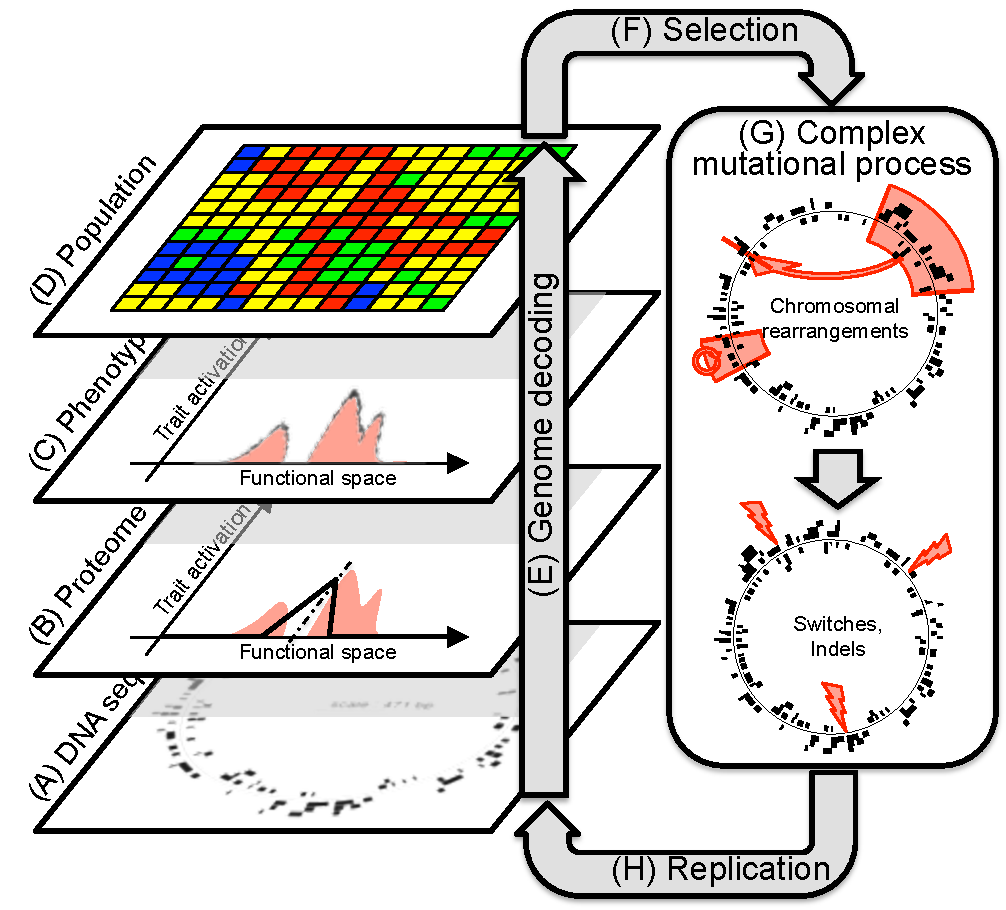
\includegraphics[width=\textwidth]{aevol/images/aevol.pdf}
\caption[Overview of the \emph{Aevol} model]{Broad overview of the \emph{Aevol} model.
\emph{Aevol} applies an evaluation-selection-replication evolutionary loop to a population of individuals defined by their genome, encoded as a circular string of nucleotides (A, central ring), on which RNA sequences and genes are decoded (A, black segments).
The resulting proteins (B, in black) are mapped to an abstract phenotypic space, and summed in order to obtain the phenotype of the individual (C, in black), which is compared to an optimal phenotype (that implicitly represents the environment -- B and C, in pink), in order to compute its fitness.
In the model, the population is laid out on a square grid (D), with one individual per cell.
In order to produce a new generation, the ancestor of the new individual in each cell is chosen at random among the neighboring individuals, proportionally to their fitness (F).
Once this ancestor is chosen, its genome undergoes a series of random mutations, including rearrangements and local mutations (G), in order to obtain the genome of the new individual in the cell at the next generation (H).
}
\label{fig:aevol:model}
\end{figure}

\subsection{Overview}

The \emph{Aevol} platform, developed in the Inria Beagle team~\citep{rutten2019}, is a software suite designed to run artificial evolution experiments on a computer, rather than at the bench.
It was originally created to investigate the influence of classical population genetics parameters such as population size, mutation rate, or selection pressure on genomes themselves, seen as an integral part of the phenotype and not only as the source of genetic information; in \emph{Aevol}, individuals have a very abstract phenotype, in exchange for a genome that is modeled down to the nucleotide level, and follows the ``central dogma of molecular biology''~\citep{crick1958}, with an accurate representation of RNA transcription and gene translation.
This approach contrasts with other artificial evolution platforms such as \emph{Avida}~\citep{adami1994,ofria2004}, which aim at studying the evolutionary process itself, rather than its impact on biological organisms.
\emph{Aevol} has for instance been used to study the effect of mutation rate on genome size~\citep{knibbe2005}, or of the selection pressure on the percentage of non-coding bases and number of genes on the genome~\citep{batut2013}.
As an excellent and very thorough description of \emph{Aevol} (in French) can be found in~\cite{liard2020b}, the following presentation of the model will be kept short and to the point.
Figure~\ref{fig:aevol:model} provides a comprehensive overview of the evolutionary algorithm at the core of \emph{Aevol}.

\subsection{The Genotype-Phenotype Map in \emph{Aevol}}

A genome or genotype in \emph{Aevol} consists in a sequence of binary characters ($0$ or $1$), which represent a double-stranded circular sequence of DNA.
The genome sequence explicitly describes the first (forward) strand of DNA, while the second (reverse) strand is obtained by taking the complement of the sequence, replacing $0$ by $1$ and vice-versa.
In order to turn this genotype into a phenotype (Figure~\ref{fig:aevol:model} C), the decoding algorithm starts by looking for sequences that code for RNAs, reading the forward strand left-to-right and the reverse strand right-to-left.
An RNA starts with a promoter sequence, which has to match a consensus sequence with up to $d_{max}$ errors, and ends with a hairpin-like terminator.
Then, each RNA is scanned for genes, which start with a ribosome binding site followed by a 3-nucleotide start codon.
Reading continues until a stop codon is found in the same frame, and the resulting string of codons is then translated into a protein, or discarded if no stop codon is found in frame before the end of the RNA sequence.
An RNA can thus contain zero, one, or several protein-coding genes.

As the genetic alphabet is binary in \emph{Aevol}, there are 8 different 3-nucleotide codons, and 6 codons can therefore be used to encode protein data, on top of the start and stop codons.
These codons are grouped into three pairs, each respectively encoding the width $w$, height $h$, and mean position $m$ of a triangle kernel function from $[0, 1]$ to $[0, 1]$ (as represented in Figure~\ref{fig:aevol:model} B).
The mean $m$ represents the main function that the protein fulfills in the abstract phenotypic space, the height $h$ the intensity with which it does, and the width $w$ the pleiotropic ability of the protein to fulfill neighboring phenotypic functions.

In order to obtain the final contribution of the protein to the phenotype, the constitutive height $h$ of the gene is weighted by the expression level $e$ of the RNA that carries the gene, which depends on the activity of the promoter of that RNA.
In the model, the promoter activity decreases linearly with the difference $d$ between its sequence and the consensus sequence, and vanishes at $d=d_{max}$.
The expression level of the RNA is then finally given by the following equation: $e = 1 - \frac{d}{1+d_{max}}$.
Finally, in order to compute the complete phenotype of the individual from the set of its proteins, the kernel functions representing each gene are summed, resulting in a piecewise-linear phenotype function.
As the maximum degree to which each phenotypic function can be fulfilled is bound to 1, the phenotype function is finally capped using Łukasiewicz operators in order to keep within this limit.

\subsection{Fitness}

Once the phenotype of an individual has been decoded from its genome, we can compute its fitness.
As the environment is indirectly specified by an optimal phenotype, we first compute a phenotypic gap as the integral of the absolute value of the difference between the phenotype of the individual and the optimal phenotype, taken over the range of phenotypic values (the $L^1$ distance between the functions).
Then, we compute the fitness as the inverse exponential of the phenotypic gap, multiplied by a selection coefficient: the higher the coefficient, the larger the difference in fitness between individuals with the same difference in gap.

\subsection{Mutational Operators}

Once the ancestor of a new individual has been chosen, a set of random mutations are applied to its genome to obtain the new genome.
These mutations are split in two classes, depending on the proportion of the genome that they can affect: genomic rearrangements, and local mutations.

Genomic rearrangements can affect up to the whole genome, and comprise four kinds of structural changes: duplications, deletions, inversions, and translocations.
In each of these rearrangements, the two endpoints of the affected segment are first drawn randomly on the genome.
In a large duplication, an additional insertion point are randomly selected on the genome, and the genetic content located between the endpoints is copied at the insertion point.
In a large deletion, the genetic content between the endpoints is simply discarded.
In an inversion, the segment is reinserted left-to-right between the endpoints, reversing the orientation of every gene located on the inversion.
Finally, in a translocation, the genetic content is removed, turned into a circular plasmid, cut at a random point in the plasmid, and reinserted at another insertion point in the genome.

Local mutations, on the contrary, comprise small insertions, small  deletions (collectively known as indels), and switches.
In a small insertion or deletion, up to 6 contiguous bases are either inserted (choosing each base at random) or deleted at a random point in the genome.
In a switch, the value of a random nucleotide is switched, from 1 to 0 or vice-versa.


\section{Modeling DNA Supercoiling in \emph{Aevol}}
\label{sec:aevol:aevol_sc}

In order to model the effect of supercoiling on gene transcription in \emph{Aevol} I chose to start with very simple approximations,
both for the level of supercoiling itself and for its effect on transcription, as the \emph{Aevol} model is already quite complex by itself.

\begin{figure}
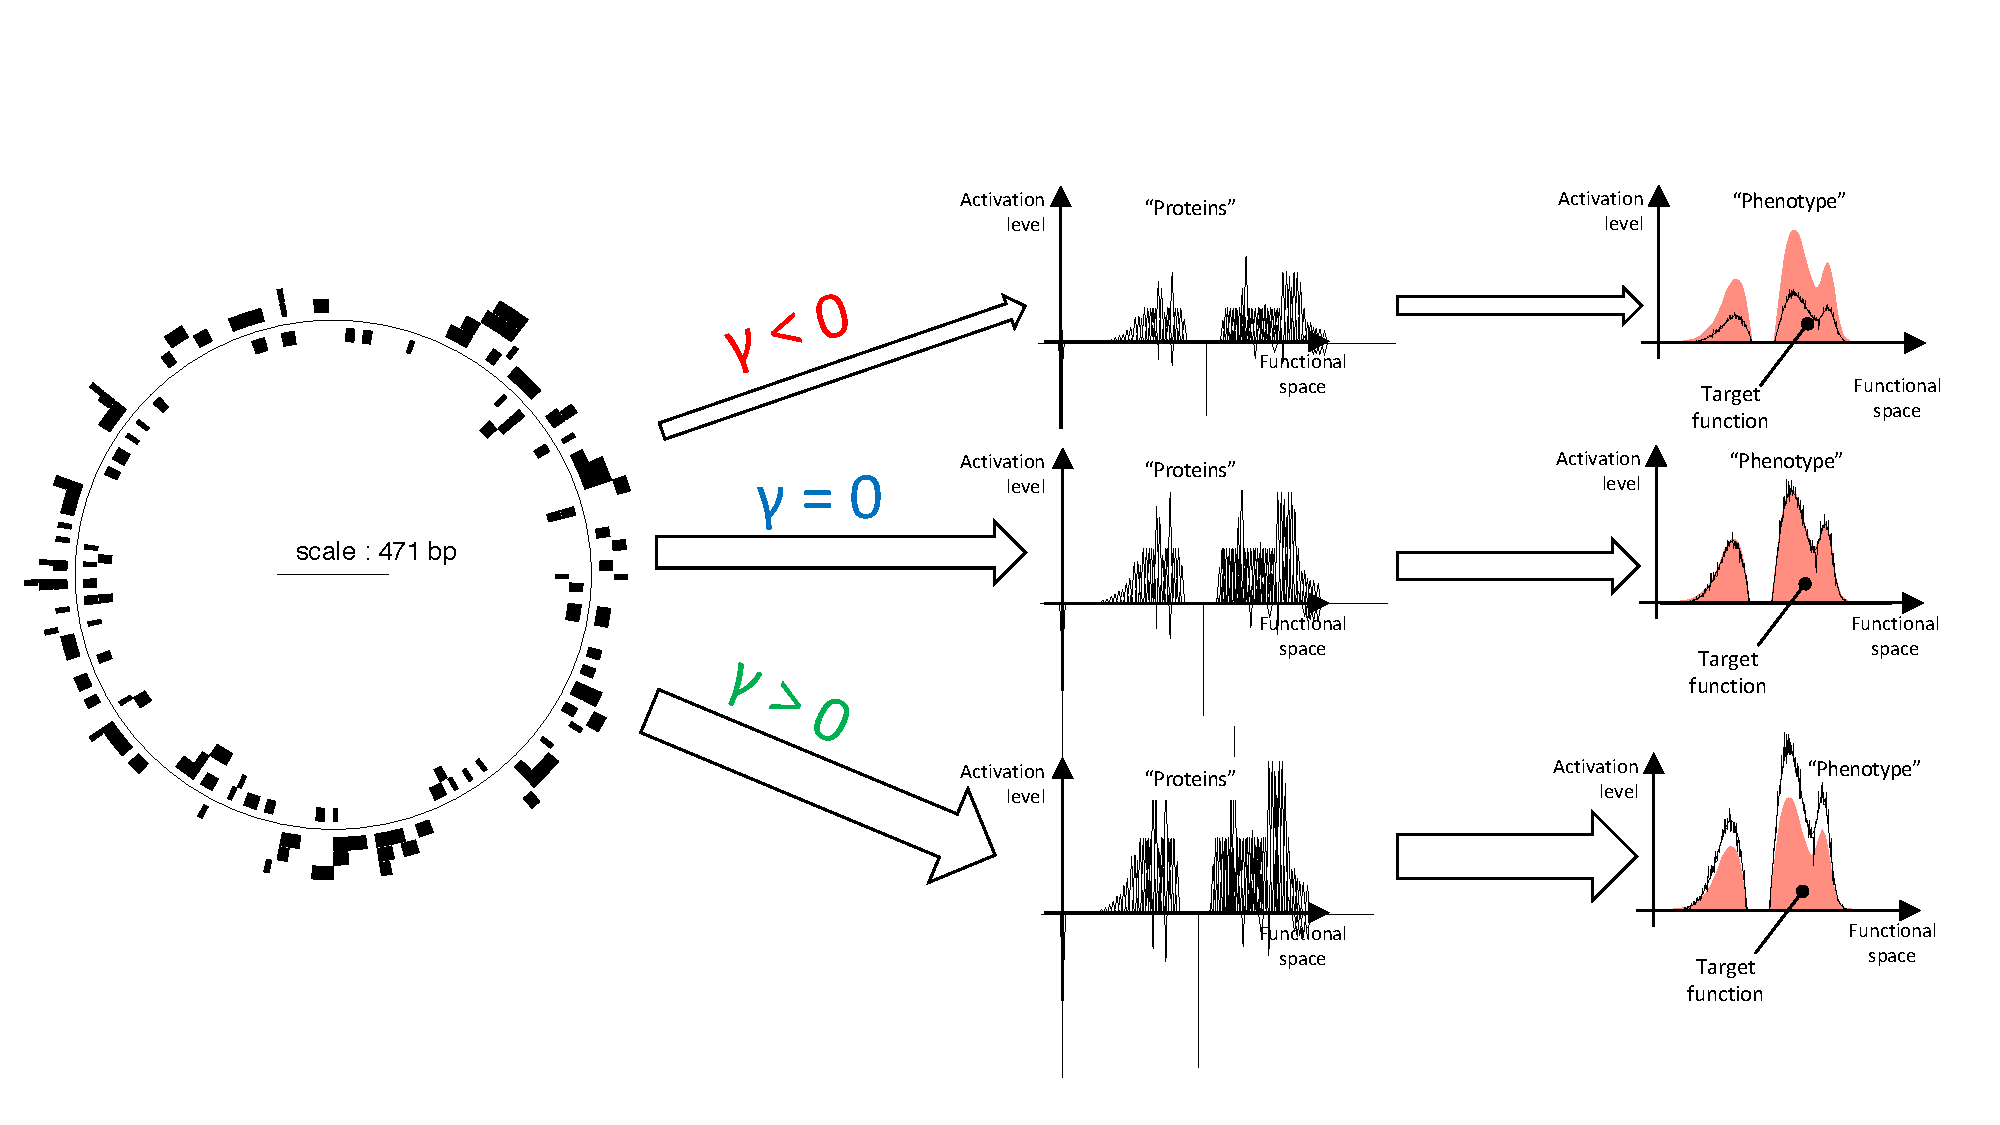
\includegraphics[width=\textwidth]{aevol/images/supercoiling_aevol.pdf}
\caption[Effect of supercoiling on the phenotype of an individual in \emph{Aevol}]{Effect of supercoiling on the phenotype of an \emph{Aevol} individual.
Left: genome (central ring) and genes (black rectangles) of the individual.
Middle: kernel function encoded by every gene in the phenotypic space, affected by an excess of positive supercoiling (top), no extra supercoiling (middle), or an excess of negative supercoiling (bottom).
Right: phenotype of the individual in each situation, compared to the optimal phenotype (in pink).}
\label{fig:aevol:sc_phenotype}
\end{figure}

\subsection{Level of DNA Supercoiling}
First, I consider the supercoiling level as constant along the genome and over time, which can be interpreted as taking the spatial and temporal average of the (actually dynamic) supercoiling level.
To implement this model inside \emph{Aevol}, I changed the genotype of individuals by adding, alongside the string-of-nucleotides genome, a single parameter $\gamma$ which represents the relative variation in the supercoiling level $\sigma$ of this individual compared to a reference supercoiling level $\sigma_0$: $\gamma = \frac{\sigma-\sigma_0}{\sigma_0}$.

\subsection{Gene Expression}
To keep the model as simple as possible, I also chose to model the effect of supercoiling on transcription as having the same linear effect on the transcription rate of every RNA on the genome.
I therefore updated the computation of the gene expression $e$ to take supercoiling into account, in addition to promoter activity:

\begin{equation}
e = (1 - \frac{d}{1+d_{max}}) \cdot (1 + \gamma)
\label{eq:aevol:sc}
\end{equation}

The effect of supercoiling on the phenotype of an example (pre-evolved) individual in the model is presented in Figure~\ref{fig:aevol:sc_phenotype}.
When $\gamma < 0$ (top row), that is when there is an excess of positive supercoiling compared to the baseline, the expression of every gene is decreased.
When $\gamma$ is equal to 0 (middle row), the supercoiling level is equal to the baseline, resulting in no change to gene expression levels, and replicating the behavior of the original \emph{Aevol} model.
Finally, when $\gamma > 0$ (bottom row), that is when supercoiling is more negative than the baseline, the expression of every gene is increased.

\subsection{Mutational Operator}
\label{sec:aevol:mut-sc}

In biological organisms, the supercoiling level is only a direct property of the DNA molecule, but is also controlled by topoisomerases and nucleoid-associated proteins that are not modeled in \emph{Aevol} (as the phenotypic space is completely abstract), and changes in the supercoiling level come from mutations affecting the genes that encode these proteins, such as \emph{gyrA} or \emph{fis}~\citep{crozat2005}.
In order to model mutations in the supercoiling level in \emph{Aevol}, I chose a continuous model, in which a small variation in $\gamma$ indirectly reflects the effect of a mutation in one of the supercoiling-controlling genes.

When an individual reproduces, we first use a Bernoulli trial, with a probability $p$ that represents the probability that a supercoiling-protein gene undergoes a non-synonymous mutation, to decide whether to change the supercoiling level.
Then, if the supercoiling level should change, we draw a variation in relative supercoiling $\Delta\gamma$ according to a normal distribution $\mathcal{N}(0, s^2)$, and finally set the relative supercoiling level $\gamma'$ of the offspring to $\gamma' = \gamma + \Delta\gamma$.
The parameters of these laws are parameters of the simulation, and their values are given in Table~\ref{tab:aevol:param_values}.
Throughout this chapter, I will for clarity refer to the usual DNA-affecting mutations presented in~\ref{sec:aevol:model} as \emph{genomic mutations}, and to the mutations in the supercoiling level presented here as \emph{supercoiling mutations}.


\section{Results}
\label{sec:aevol:results}

As presented in the introduction of this chapter, the goal of implementing a supercoiling model in \emph{Aevol} was twofold.
The first aim was to see to which extent adding a new dimension to the phenotypic space, and a new mutational operator to explore this new dimension, would allow populations to evolve faster than allowed by the original model, thank to the wide jumps in the phenotypic landscape made possible by the supercoiling mutations.
The second aim was to disentangle the possible epistatic effects between supercoiling mutations and genomic mutations in \emph{Aevol}.
In this section, I first present the experimental setup that I used in order to answer these questions.
Then, I show that adding regulation by supercoiling did not measurably increase the rate of adaptation of the populations compared to the control, and that supercoiling indeed follows a very constrained evolutionary trajectory in these experiments.
Finally, I conclude that I could not find any observable epistasis between supercoiling and other mutations, when using the supercoiling model presented in Section~\ref{sec:aevol:model}.

\subsection{Experimental Setup}

In order to tackle these questions, I ran two sets of simulations: the experimental runs using the supercoiling model, and the control runs using the vanilla version of \emph{Aevol}.
Each set of runs comprises 5 replicate populations, which were evolved for 1,000,000 generations, each starting from a clonal population.
Each of the initial individuals were obtained by randomly drawing 5,000 bp-long genomes, until a genome with a non-zero fitness (i.e., at least one protein-coding gene partially matching the phenotypic target) was found.
The simulations were run on a 24-core Intel(R) Xeon(R) CPU E5-2620 v3 @ 2.40GHz server with 128 GB of RAM, and lasted approximately a week for each set of replicates.
The limited number of replicates for each set of simulations was chosen to balance their energy expenditure with the preliminary character of the work, which alleviates the need for statistical strength in the resulting data.

\subsection{Studying Lineages}

The data that is presented in the rest of this section was obtained by reconstructing the lineage, starting from the initial generation, of a random individual at the last generation of each replicate.
Studying a given lineage, rather than the best individual at every generation (which need not sire one another), allows us to reconstruct the precise set of mutations that happened throughout the evolutionary history of this lineage, and therefore gives us information about the possible causal link between these mutations, and hence about their possible epistatic relationships.

As a theoretical haploid Wright-Fisher population with $N$ individuals coalesces on average in $2N$ generations without mutation or selection~\citep{felsenstein2019}, we chose to analyze the data from generation 0 to 990,000 of every replicate (excluding the last 10,000 generations), ensuring that each lineage is indeed ancestral to the whole population of the last generation of that replicate.

\begin{table}
  \begin{center}
    \begin{tabular}{ l r r }
    \toprule
    \textbf{Parameter} & \textbf{Symbol} & \textbf{Value}\\
    \midrule
    Population size & N & 1,024 (32x32 grid) \\
    Initial genome size & $g_0$ & 5,000 bp \\
    Local mutation rate & $\mu_{loc}$ & $10^{-7}$ bp$^{-1}$.gen$^{-1}$ \\
    Rearrangement rate & $\mu_{rear}$ &$10^{-6}$ bp$^{-1}$.gen$^{-1}$ \\
    \midrule
    Initial supercoiling level & $\gamma_0$ & 0 \\
    Supercoiling mutation probability & $p$ & $10^{-1}$ \\
    Supercoiling mutation variance & $s^2$ & $10^{-2}$ \\
    \midrule
    Generations & T & 1,000,000 \\
    Number of replicates & $n$ & 5\\
    \bottomrule
    \end{tabular}
    \end{center}
  \caption[Table of parameter values for the \emph{Aevol} runs]{Table of parameter values used in the \emph{Aevol} evolutionary runs.
  The top part describes parameters common to the experimental and control set of rules, the middle part the supercoiling-related parameters introduced in the supercoiling model, and the bottom part the simulation parameters.}
  \label{tab:aevol:param_values}
\end{table}


\subsection{Evolution of the Fitness Level}

\begin{figure}
  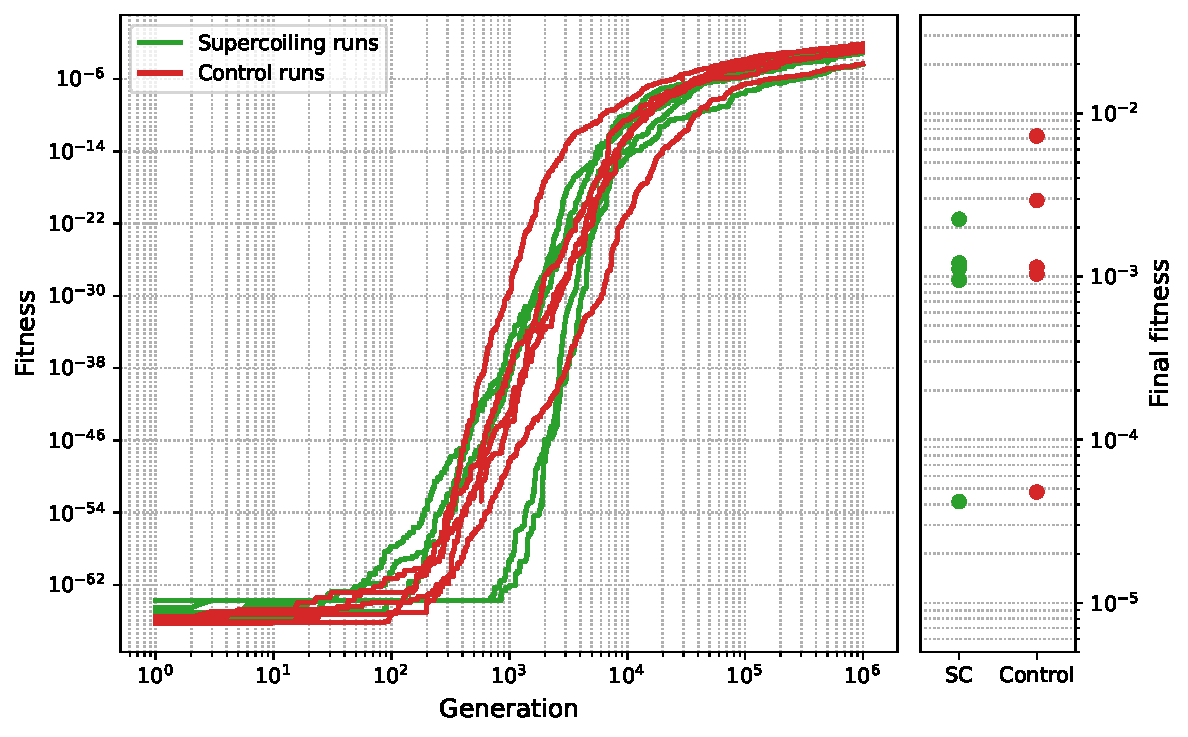
\includegraphics[width=\textwidth]{aevol/images/fitness_all.pdf}
  \caption[Evolution of the fitness of the control and experimental runs in \emph{Aevol}]{Left: Evolution of the fitness at every generation throughout the lineage of the final population of each replicate of the experimental (green) and control (red) runs.
  Both axes follow logarithmic scales.
  Right: Fitness of the lineage individual at the 990,000th generation of each run, separated between supercoiling (green) and control (red) runs.}
  \label{fig:aevol:fitness}
\end{figure}

Figure~\ref{fig:aevol:fitness} presents, on the left-hand side, the fitness of the individual at every generation of the lineage of the final population, or lineage individual, in each replicate.
In each case, the fitness follows a broadly sigmoid shape (note that both axes are logarithmic): fitnesses quickly increase from generation 100 up to generation 100,000, then slow down for the remaining 900,000 generations, but never completely cease to progress, mirroring in \emph{Aevol} the open-ended evolution observed in the LTEE.
The right-hand side of Figure~\ref{fig:aevol:fitness} shows the fitness of the lineage individual at the 990,000th generation of each run.

With the limited number of replicates of each run, there is no discernible difference in fitness between the two experimental conditions, with and without mutations in the supercoiling level.
Adding the new phenotypic dimension of the supercoiling level, and the associated supercoiling mutational operator, therefore does not seem to play an important role in the rate of evolution of the populations modeled in \emph{Aevol}.

\subsection{Evolution of the Supercoiling Level}

\begin{figure}
  \centering
  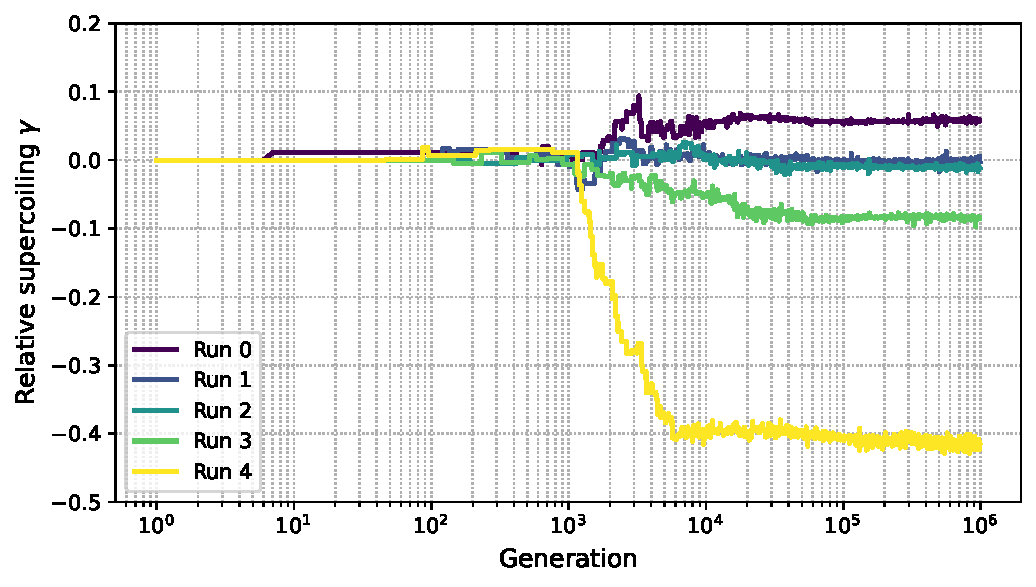
\includegraphics[width=0.9\textwidth]{aevol/images/supercoiling_all.pdf}
  \caption[Evolution of the supercoiling level of the experimental runs in \emph{Aevol}]{Evolution of the relative level of supercoiling at every generation of the lineage of each of the experimental runs.}
  \label{fig:aevol:sc}
\end{figure}

Figure~\ref{fig:aevol:sc} shows the evolution of the supercoiling level throughout the lineage in each of the 5 replicates.
In every run, the supercoiling level evolves only at the very beginning of the run, stabilizing in a few tens of thousands of generations, and remains essentially constant afterwards.
This is in strong contrast to the fitness of the runs (presented in Figure~\ref{fig:aevol:sc}), which keep increasing until the end of the runs.

It therefore seems that the supercoiling level might play a role in the early evolution of the runs, but not in their long-term fitness improvement.
This result is in a sense slightly disappointing but was not entirely unexpected.
Indeed, in the early evolution of individuals in \emph{Aevol}, the phenotypic target is only very imperfectly approached by the proteins expressed by the individual.
At that stage, mutations in the supercoiling level, which affect the expression level of every protein equally, could indeed have a positive effect by bringing the whole phenotype closer to the optimum, in a very broad swipe.
Indeed, as individuals in \emph{Aevol} evolve from an ancestor with a single good gene, phenotypic functions are often under-performed by individuals at the early stages of evolution in the model, as the width and height of the kernel functions of their genes can be small, and as the expression level of their RNAs can be quite low if their promoters contain too many errors.
The different supercoiling value towards which each of the replicates tends to converge in Figure~\ref{fig:aevol:sc} could therefore be interpreted as a founding effect coming from the genome of the original individual in that run, which could be confirmed by a more detailed analysis of the series of mutations that happened in each lineage.

However, as evolution progresses, and as the optimal phenotype is more and more closely matched by the individual, changing the whole expression profile at once becomes less and less susceptible to be favorable.
This case is represented in Figure~\ref{fig:aevol:sc_phenotype}: any change in supercoiling, be it positive or negative, will decrease the fitness of the individual, and supercoiling mutations are therefore less and less susceptible to be picked up in the lineage.

These results tend to show that the model in which supercoiling has a global, linear effect on gene expression levels is too simplistic in order to produce phenotypic effects that are variable enough to have a chance to be picked up by selection; and therefore that this model is insufficient to study the interplay between supercoiling mutations and genomic mutations in \emph{Aevol}.

\subsection{Looking for Epistasis}

\paragraph{Waiting Times Before and After Mutations}
In order to detect signs of positive or negative epistasis between the different kinds of mutations, I used the following approach, which considers the waiting times before and after mutations happen:
if, for a given mutation type, the average time until a new favorable mutation fixes in the lineage after a mutation of that type is smaller than the average time since the last favorable mutation before that mutation, this could be interpreted as a sign that the mutation has increased the probability of a favorable mutation happening; in other terms, as a broadening of the evolutionary paths available to the genome, or a sign of positive epistasis between that kind of mutation and other kinds of mutations.
On the contrary, if it takes longer for a new favorable mutation to fix in the lineage after that mutation, it would be a sign that the evolutionary paths have been constrained by the inversion, or as a sign of negative epistasis.

The data obtained following this approach is presented in Figure~\ref{fig:aevol:epistasis}.
For each mutation type, it shows the average number of mutations of that type that fixed in the lineage of each replicate, as well as the average time after which a mutation of that types fixes after a non-neutral mutation (left), and before a non-neutral mutation fixes after a mutation of that type (right), in the control runs (top) and in the experimental runs (bottom).

\paragraph{Epistasis of Duplications and Deletions}
In the control, a faint pattern seems to be discernible for large-scale inversions and deletions: the average time to a new mutation after a deletion is slightly higher than the time before a deletion, hinting that deletions could present a negative epistasis with other mutations.
Conversely, the time to a new mutation after a duplication is slightly lower than the time before the mutation, hinting that duplications could on the contrary present positive epistasis with other mutations.
Local mutations, as well as rearrangements and inversions, do however not seem to swing one way or the other.

In the experimental runs, no such pattern is visible at first sight, including for the supercoiling mutations, and the global average waiting times are smaller than in the control, which is consistent with the introduction of a new mutation type.
There therefore seems to be no sign of epistasis between the supercoiling mutations and the genomic mutations, when following the approach explained above.

\begin{figure}
  \centering
  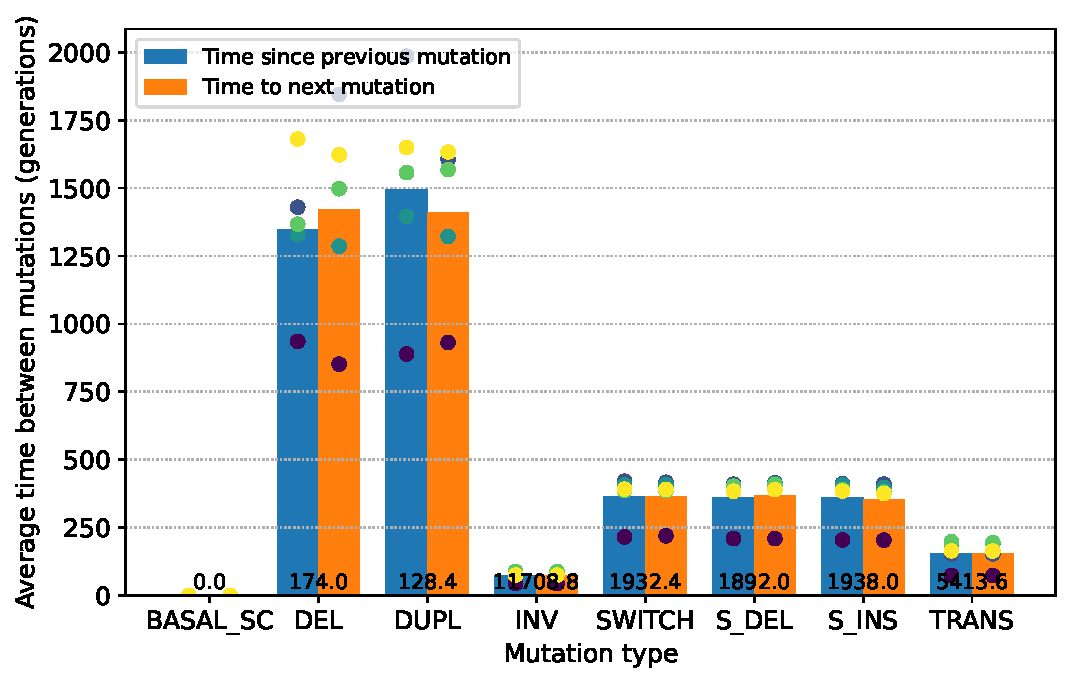
\includegraphics[width=0.9\textwidth]{aevol/images/epistasis_control.pdf}
  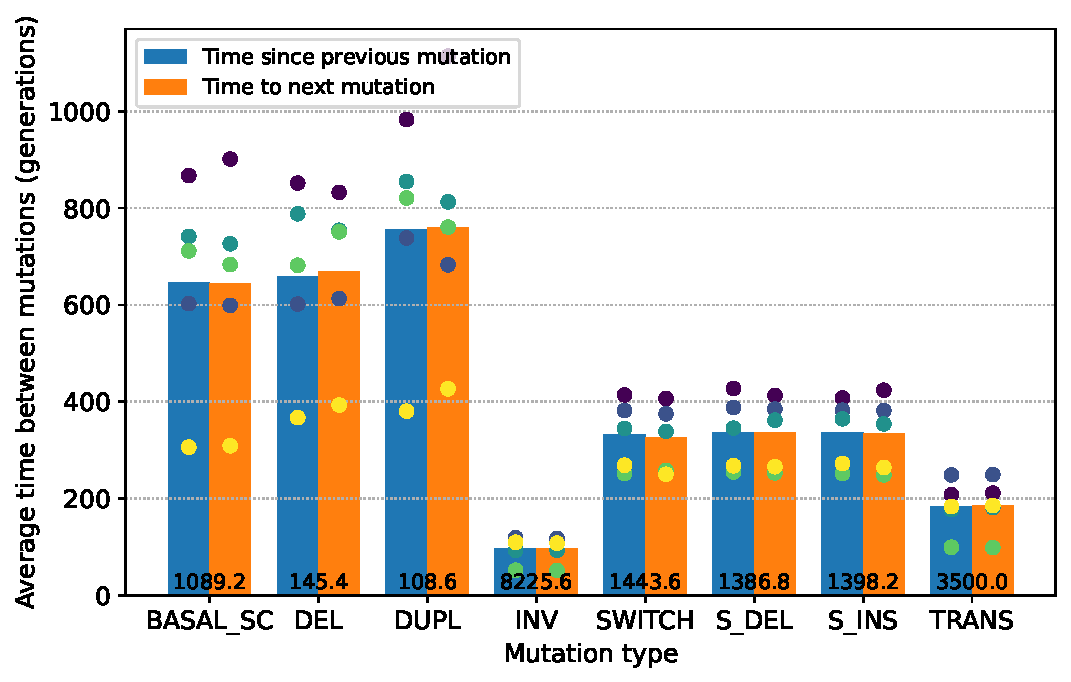
\includegraphics[width=0.9\textwidth]{aevol/images/epistasis_sc.pdf}
  \caption[Measuring epistasis with the average times before and after mutations]{Average time before and after a mutation of each kind, in the control runs (top) and the experimental runs (bottom).
  For each kind of mutation, the times presented show the wait time until a neutral mutation of that kind after a non-neutral mutation of any kind, and the time until the next non-neutral mutation of any kind after a mutation of that kind.
  The bars show the average over the five replicates, and the colored dots are the value for every replicate.
  The average number of neutral mutations of each type is displayed at the bottom of the corresponding bar.}
  \label{fig:aevol:epistasis}
\end{figure}

\paragraph{Role of the Genome Size}
A hypothesis that could explain the pattern visible in the control runs for the large deletions and duplications is that the difference in waiting times, and hence the positive or negative epistasis, is simply due to the change in the genome size caused by this mutations.
All mutation rates in the model are indeed proportional to the genome size, and the expected number of mutations at each generation therefore increases and decreases with the genome size (assuming that there is no fitness effect or selection).
However, in the experimental runs, the probability of a supercoiling mutation importantly does not depend on the genome size.
A hypothesis to explain the disappearance of the signal (possibly) present in the control for duplications and deletions could therefore be that supercoiling mutations tick according to their own clock, which depends on their parameters $p$ and $s^2$, but not on the state of the genome itself.
For example, if a certain beneficial indel is allowed to happen because of a duplication and indeed happens sometime after that duplication in the lineage, but a supercoiling mutation has happened between the duplication and the indel, then the signal from this particular epistatic relationship will have been hidden by that supercoiling mutation.

\section{Conclusion}
\label{sec:aevol:ccl}

The goal of this initial work was to study the ways in which supercoiling mutations affect the fitness landscape of individuals in \emph{Aevol}, that is the possible epistatic interactions between supercoiling mutations and other kinds of mutations.
In order to tackle this question, I implemented a model of the effect of the supercoiling level on gene expression, as well as a model of mutations in the supercoiling level, in \emph{Aevol}.
Using this version of the model, I ran evolutionary experiments, in which I compared the evolution of populations with supercoiling with control populations by analyzing the fitness, supercoiling level, and mutations fixed in the lineage of individuals that leads to the final population of every replicate.

With the limited data available, I could not find a difference in the evolution rates of each set of experiments, and deduced that supercoiling does not seem to play an important evolutionary role in this model; this result was substantiated by the fact that the supercoiling level converges very quickly to a fixed level in the evolutionary history of each population.
I then tried to detect signals of positive or negative epistasis between the different kinds of mutations, by looking at the waiting times between each kind of mutation.
While this approach did not lead to meaningful results in the experimental runs, it did hint at a possible epistatic link between duplications or deletions and the other mutation kinds, due to their effect on genome size, in the control runs, which seems promising to further investigation.

\paragraph{}
The verdict of these preliminary experiments was that the model of supercoiling that I implemented in \emph{Aevol}, in which supercoiling is kept constant along the genome and affects the expression level of all genes equally, was probably too simplistic to obtain meaningful results as-is.
Rather than pursuing this avenue of research further by implementing a more precise model in \emph{Aevol}, I chose instead to go in a different direction.
In order to decouple the complexity of the \emph{Aevol} model from the study of the evolutionary role of supercoiling, I decided to simplify the individual model, genotype-phenotype map, and mutational operators as much as possible, in order to model the effect of supercoiling on gene expression more precisely while keeping the overall complexity of the model in check.
The results of this renewed approach are presented in the following chapters.